%!TEX root = Thesis_main.tex
\chapter{Introduction}
\label{chapter1}
\begin{figure}
	\centering
	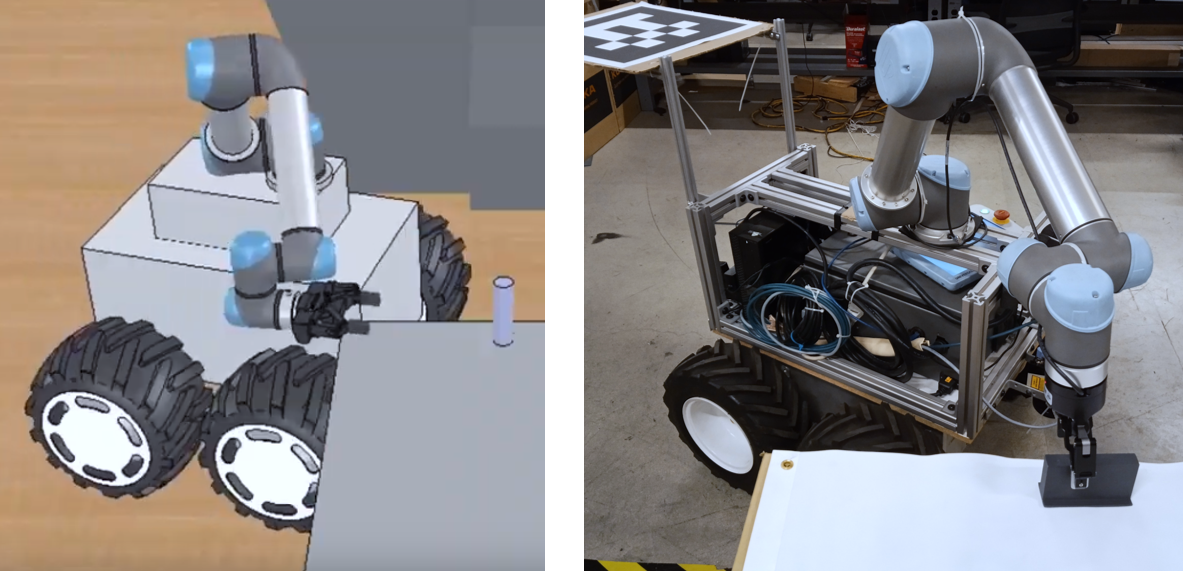
\includegraphics[scale=0.5]{MM}
	\caption{The Mobile Manipulator at the USC Center for Advanced Maufacturing}
	\label{fig:MM}
\end{figure}
In the last decades industry is being moving from the use of traditional robotic manipulator arms, which executes highly specific simple tasks in controlled and secure environments, like spot welding, towards more complex and flexible robotic systems, which should be able to cope with dynamic and uncertain environments, until nowadays where different types of mobile robots can be found in a great variety of environments, ranging from the cleaning robots in people houses, to the rovers exploring the outer space (Figure \ref{JPL_rover}). In particular the past few decades have seen a gradual increase in the use of autonomous Mobile Manipulators in a wide variety of applications, such as machine tending, transportation of parts on a shop floor, and inspection of large aerospace parts. Mobile Manipulators combine a mobile base and one or more robotic arms, combining locomotion and manipulation capabilities in order to the fulfillment of the forementioned missions. These operations require the Mobile Manipulator to follow complex trajectories in highly cluttered environments while satisfying constraints on joint velocity and joint limits.
\begin{figure}[t]
	\centering
	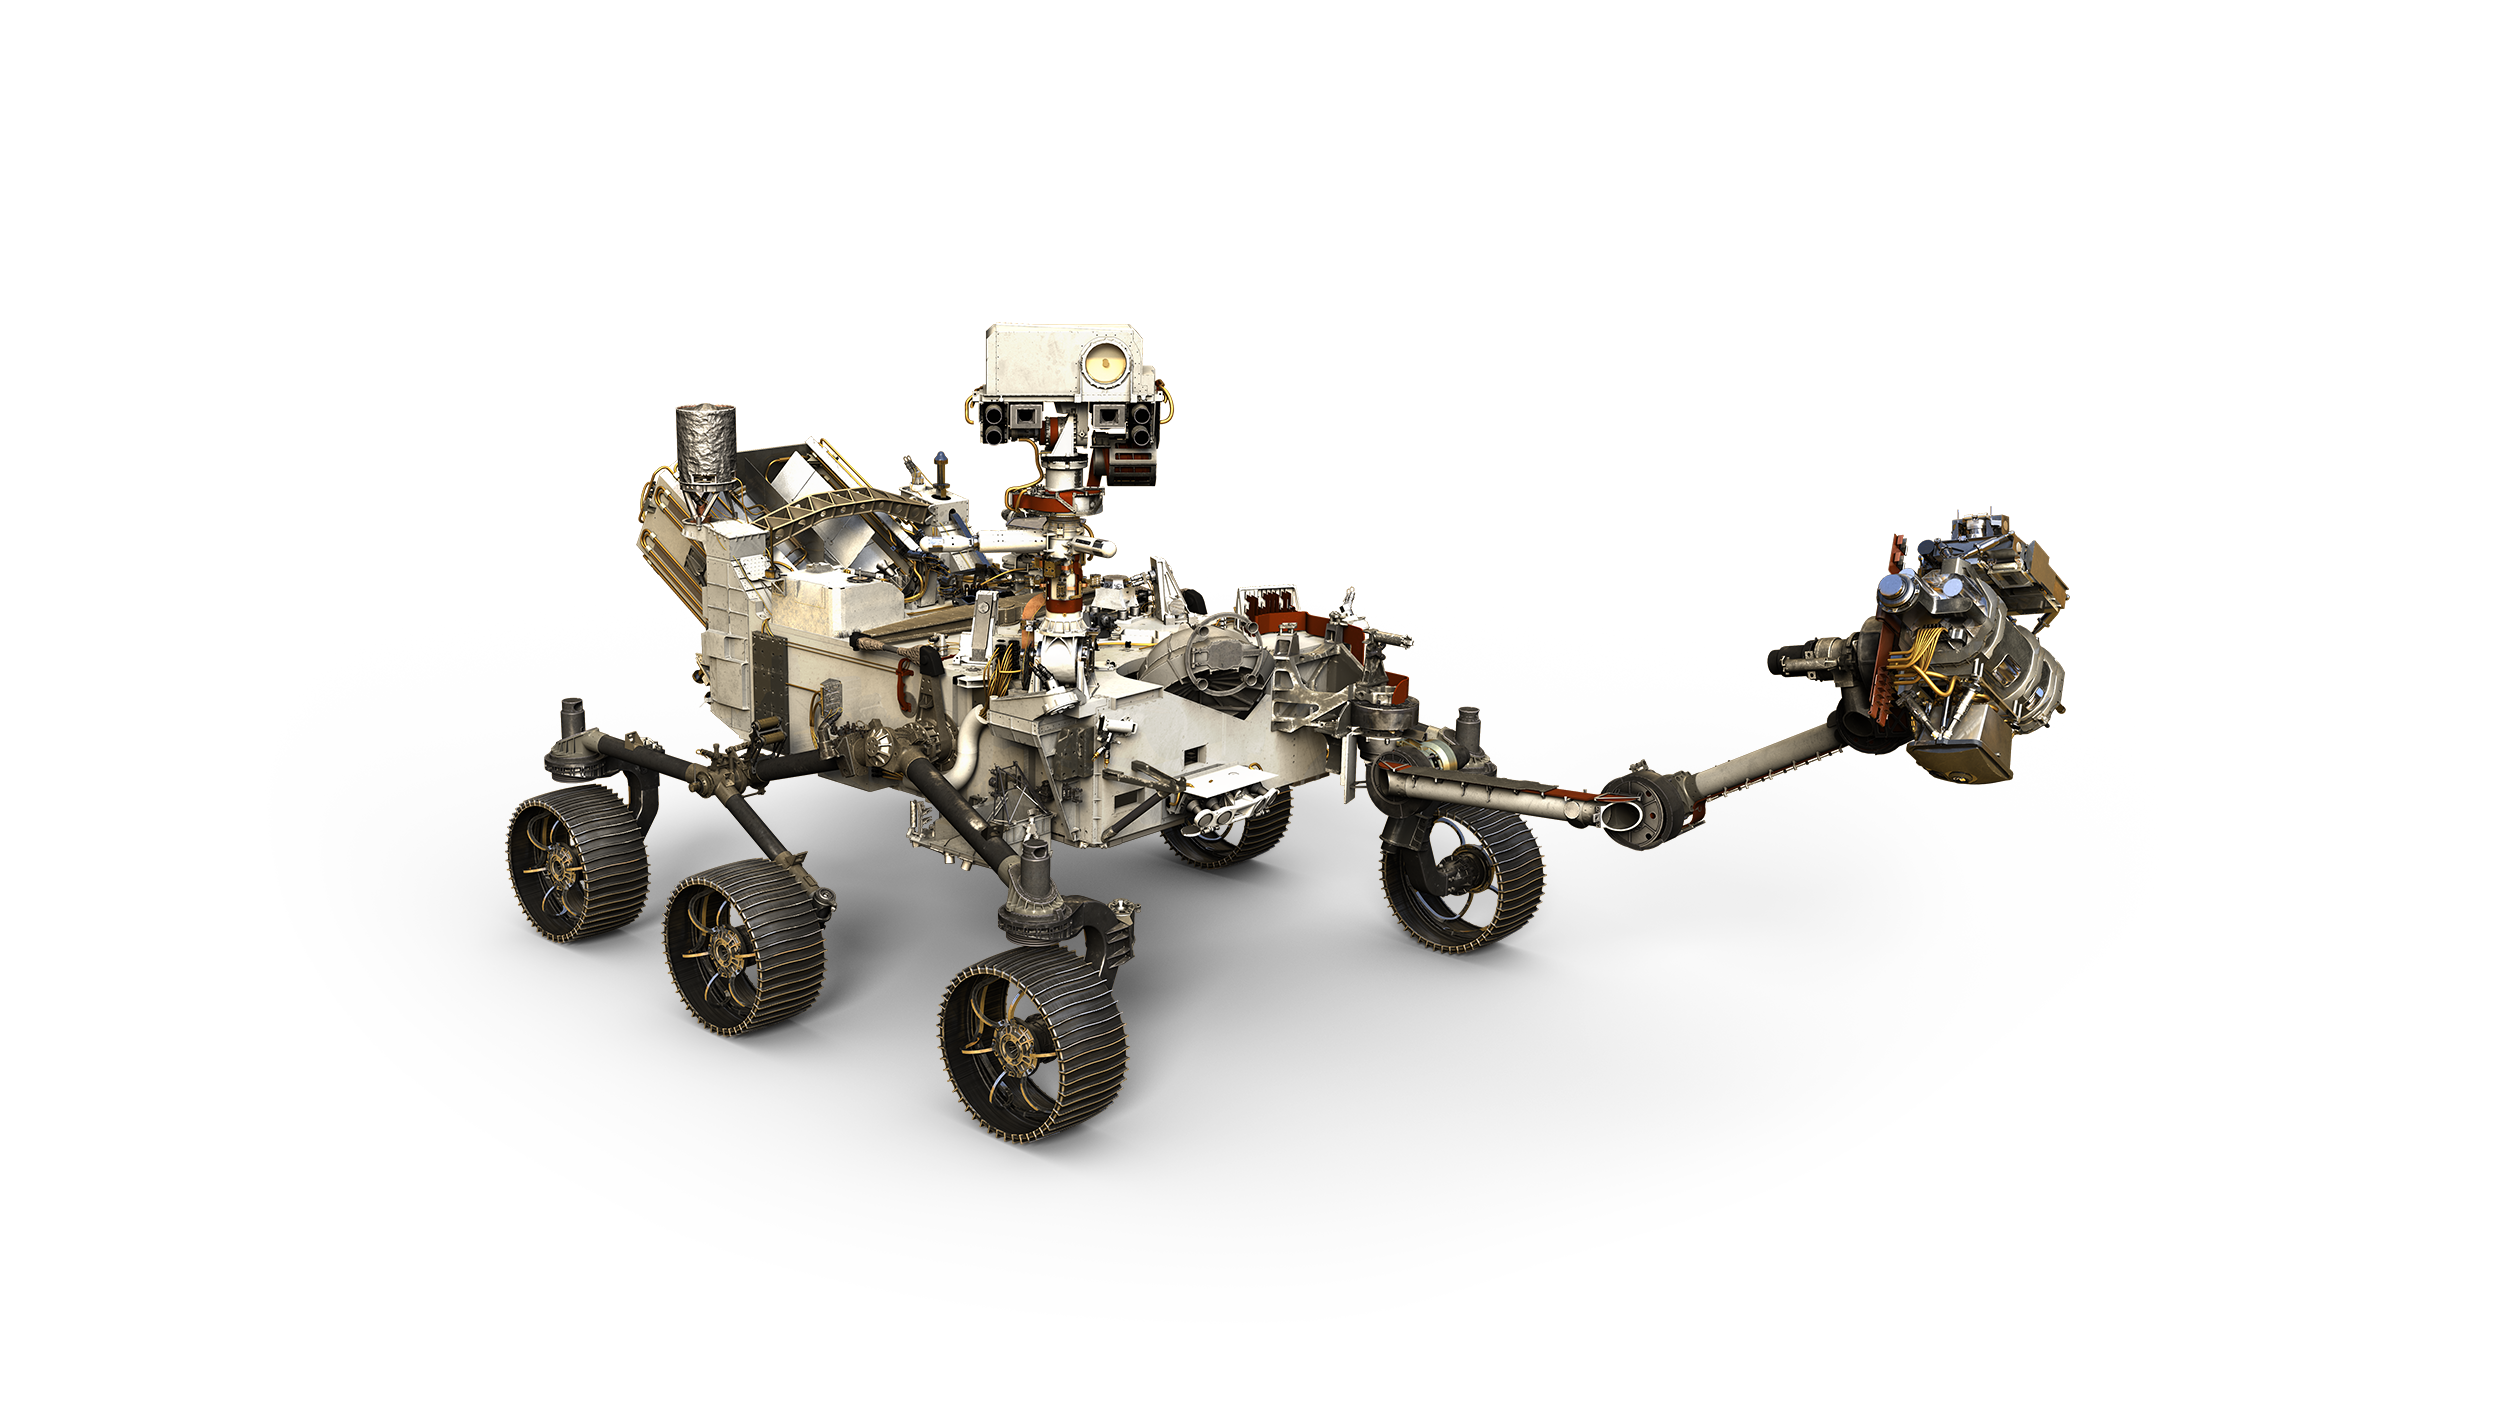
\includegraphics[scale=0.12]{JPL_rover}
	\caption{JPL Rover designed for Mars2020 mission}
	\label{JPL_rover}
\end{figure}
%Fig. \ref{fig:MM_image} illustrates examples where a mobile manipulator needs to move the end-effector along a specific trajectory in order to complete the task. Fig. \ref{fig:MM_image}(a) shows our physical platform ADAMMS (Agile Dexterous Autonomous Mobile Manipulation System) while picking up objects. Examples of a mobile manipulator carrying a long rod through a cluttered environment and picking up objects while moving is shown in Figs. \ref{fig:MM_image}(b) and (c). 
In such situations, trajectories are typically generated in a hierarchical manner. In the first layer, an optimal reference trajectory is computed and, in a second layer, this trajectory is tracked using a trajectory tracking controller.\\
In order to minimize trajectory execution time, that is usually the goal of the control system, the manipulator and the mobile base need to move in a synchronized fashion; this requires reasoning in high-dimensional state spaces.
Furthermore, the motion model of a mobile manipulator is nonlinear, and perception and actuation are usually characterized by uncertainty, whose effect on the system is particularly important in highly dynamic environments.
We thus require a real-time controller that is able to handle nonlinear models, uncertainty, and constraints in high-dimensional state spaces.\\
In this work, we present an online Model Predictive Control (MPC) strategy for a nonholonomic Mobile Manipulator (Figure \ref{fig:MM}), with a focus on trajectory tracking control for motion and grasping operations in unstructured environments.\fix{dire nel particolare che l'obiettivo è quello di fare handling+grasping}
We assume a reference trajectory for the mobile base is provided by a high-level planner, as in \cite{thakar2018case,thakar2019icra,kabir2019icra,Rajendran2017}, and the desired end effector trajectory is given as well. Since trajectory tracking in grasping tasks requires the use of a nonlinear model for the description of the end effector pose, a Nonlinear MPC (NMPC) architecture is used. The main issue related to the developement of such a controller lies in the non linearity of the model and the high redundancy of the system itself. Then, in order to overcome the limitations introduced by the high computation complexity of the optimization process, a fast online implementation of the NMPC is proposed. This technique is based on two actions:
\begin{itemize}
	\item the parameterization of the control actions, to reduce the number of optimization variables, as in \cite{Howard2007};
	\item the removal of the constraints on the terminal state, which are usually necessary for the stability of the system in a classical MPC formulation, with a weighting of the MPC cost function as in \cite{alamir2018stability}. 
\end{itemize}
This approach allows to drastically reduce the computational complexity for the online computation of the controller. 
The next chapters are organized as follows: a brief description to the model of the system under study is presented in Chapter \ref{chapter2}. The system has been described kinematically without considering the nonlinearities that a dynamic model would introduce and to properly describe the actual control inputs to the system which are the joint velocities. After a general overview of the possible existing control architectures for robotic system in Chapter \ref{chapter3}, Chapter \ref{chapter4} can be referred for a fairly thorough summary of Mobile Manipulator control; even if Mobile Manipulators are a technology known from the early 90s, just a little can be found in literature on this topic. In particular, except for very few cases, MPC control has been applied only with holonomic Mobile Manipulators. This is due to the fact that this kind of control requires high computational effort, especially with highly nonlinear systems like Mobile Manipulators. MPC is a powerful tool to face all the constraints on Mobile Manipulators motion that have to be taken into account: obstacle avoidance, self collision avoidance, joint limits, joint speed limits, singular configurations avoidance, etc. exploiting also the kinematic redundancy of the system.
In Chapter \ref{chapter5} we present the architecture of the online MPC control for the nonholonomic Mobile Manipulator under study in order to achieve a trajectory following task for the manipulator's end effector while coping with the constraints previously mentioned. Particular attention is given to the modifications we introduced underlining the advantage of their implementation. In Chapter \ref{chapter7} experimental results are presented both for simulations and experiments with the real systems in the case of handling and grasping tasks. Eventually in Chapter \ref{conclusions} conclusions are drawn highlighting our main contributions and future works.	

















